\chapter{Identification of drug response properties and methods of tissue preparation for single cell measurements in patient derived xenografts %Establishing a transplant model and the methods for single cell dissociation 
}
\label{ch:Chapter 3}

%\section{Motivation}
%Developing models that mimic human cancer is a long-standing goal in cancer research \cite{aparicio2015examining, may2018cancer, ryu2019integrative}. However, as compare to cell culture in dishes, patient derived xenograft (PDX) models better retain the biological and molecular characteristics and heterogeneity of the patient's tumor. This could be due to their close genomic and transcriptomic fidelity to the tumors of origin \cite{lin2014high}. In addition, PDX are also known as dignified models to explore patient's specific response to therapy and understanding drug resistance \cite{matossian2019drug, derose2011tumor}. So we started this chapter with the intent of establishing the transplant models of breast cancer patient derived xenografts of breast cancer to explore the baseline sensitivity patterns. This was important to select which models could be further utilized for drug resistance timeseries measurements for upcoming chapters. 

%Next, we established conditions for tissue dissociations from PDX tumors. 
%Due to the sensitivity of single-cell RNA sequencing, the data is subject to technical and biological noise \cite{potter2018single, stegle2015computational}. Moreover, small changes in gene expression can dramatically influence the interpretation of biological results. So we compared PDX tumors dissociations with different enzymes that work at different temperatures.

%Single-cell whole genome sequencing with direct library prep (DLP+) and RNA sequencing (scRNA-seq) are powerful tool for studying complex biological systems, such as tumor heterogeneity and tissue microenvironments. However, the sources of technical and biological variation in primary solid tumor tissues and patient-derived mouse xenografts for scRNA-seq are not well understood.
%Due to the sensitivity of single-cell RNA sequencing (scRNA-seq), small changes in gene expression can dramatically influence the interpretation of biological data. scRNA-seq data is also subject to technical and biological noise \cite{potter2018single, stegle2015computational} Transcriptional machinery remains active at 37\textdegree C, and extended incubation at high temperatures may introduce gene expression artifacts, independent of the biology at the time of harvest. Moreover, extended incubation at higher temperatures in the absence of nutrients or anchorage, or harsh dissociation, may induce apoptosis or anoikis, polluting the viable cell population or generating low-quality suspensions \cite{volovitz2016non}. Therefore, it is imperative to characterize the inherent variation and potential effects of cell isolation methods on the transcriptomic profiles of tissues. Recently, it has been shown that a serine protease (subtilisin A) isolated from a Himalayan glacier-resident bacterium, \textit{Bacillus lichenformis}, is suitable for dissociation of non-malignant renal tissues at 4-6 \textdegree C and can reduce scRNA-seq artifacts in these tissues, including reducing global and single-cell gene expression changes \cite{shah2012clonal}. 

\section{Synopsis}
This chapter describes the establishment and selection of PDX and drugs for study and conditions for single cell dissociation. 
 
 
 \subsection{Established transplant PDX models}
 \begin{itemize}
  \item Established 26 breast cancer patient derived xenografts (PDX) transplant models in NOD Rag-1 null interleukin-2 receptor gamma null (NRG) to assess the capabilities of tumour engraftments. 
  \item Overall engraftment rate from NSG to NRG was 90\% in total. 100\% from HR+/HER2-ve subtype,  80\% from HR-ve/HER2+ and 87.5\% from triple-negative breast cancer types (TNBC).
   \item Histology showed that PDX tumours in NRG retains their receptor status.
  
  \end{itemize}
  
 \subsection{Drug resistance and sensitivity patterns}
\begin{itemize} 
     \item First, \textit{in vitro} drug screening of patient derived xenograft tumours with 11 different chemotherapies helped selection of 4 drugs and 4 PDX  for detailed \textit{in vivo} drug studies.
     
   \item  Established qualitatively drug resistance sensitivity over 4 TNBC PDX as precursor to be used for drug resistance \textbf{\textit{in vivo}} timeseries for chapter 4.
   
 \item All 4 TNBC PDX were sensitive to cisplatin with more than 60\% tumour growth inhibition. TNBC-SA609 and SA604, having similar background mutational signature of fold back inversion (FBI), showed resistant patterns to both Rucaparib and CX-5461 with less than 30\% tumour growth inhibition. However, TNBC SA535 with BRCA 1 deficiency, was sensitive to all but partially sensitive to Rucaparib. TNBC-SA1035 was partially sensitive to Paclitaxel, resistant to Rucaparib, but sensitive to Paclitaxel and CX-5461.

\end{itemize}

 \subsection{Established conditions for single cell dissociation of PDX for downstream analysis.}
\begin{itemize} 
 
 \item Dissociation with Collagenase at 37\textdegree C induces a distinct stress response in single-cell transcriptomes
  \item Stress response genes, including \textit{FOS} and \textit{JUN}, were induced by collagenase/ hyaluronidase digestion at high temperature (37 \textdegree C), which were minimized by dissociation with a cold active protease at low temperatures (6 \textdegree C).
 \item  Subpopulations of dead, dying and live cells were identified in the transcriptomic data
  \item Cell yield from scRNAseq data was highly dependent on the cell status, with 8,597 live cells recovered but only 1,280 and 885 dead and dying, respectively, compared to targeted numbers of 3,000 cells.
   \item Dead cells exhibit significantly higher percentage of the transcriptome as mitochondrial compared to both live and dying cells
    \item The cluster of dying cells up-regulates the MHC class I gene set, suggesting it represents stressed or pre-apoptotic cells.
    \item Transcriptomic stress response was induced by both digestion time and digestion temperature.


\end{itemize}
% First, we set out to establish  breast cancer patient derived xenografts (PDX) in NOD Rag-1 null interleukin-2 receptor gamma null (NRG) mice to assess the capabilities of tumor  engraftments. Observing tumors uptake by the immunocompromised NRG host allows 
%for the identification of potential PDX which could be exposed to chemotherapies for basic sensitivity recording.

%Next, we demonstrated the efficacy of chemotherapies and the dynamic range of responses of PDX, by conducting short term \textit{in vitro} drug sensitivity assays that encouraged for \textit{in vivo} characterization of the response properties of selected conventional and targeted chemotherapies to some of the successful engrafted PDX.

%For a proof-of-principle, a modified experimental strategy of 3x1x1 for \textit{ in vivo} experiments was adopted to record the patterns of sensitivity of PDX to the drugs, taxane, platinum, PARP inhibitor and CX-5461 (G4 stabilizer). As CX-5461 was a new compound, still in clinical trial phase 11, we also tested its efficacy on some of the cell lines other than our PDX. 
 %These cell lines experiments helped in the publication of a co-authored paper in \textit{Nature Communications, 2017} \cite{xu2017cx}.
 
 %In addition to carrying out the drug sensitivity, we also needed to accomplish the effects of tumor dissociation protocols on single cell viability outcome. This was decisive because the tumors for which we characterized the drug sensitivity was destined to be used for more dynamic and advanced pre-clinical models and to submit for single cell whole genome and single cell RNA sequencing for the subsequent chapters. 
 %The PDX models for this chapter and dissociation protocols also helped in the publication of a resource paper in a co-authored publication in \textit {Cell, 2019} \cite{laks2019clonal}. 
 
 %Finally, while optimizing viability of single cells for transcriptome analysis, we found that stress response genes, including \textit{FOS} and \textit{JUN}, were induced by collagenase/ hyaluronidase digestion at high temperature (37 \textdegree C), which were minimized by dissociation with a cold active protease at low temperatures (6 \textdegree C). 
 %These findings lead to the first co-authored publication in \textit {Genome Biology, 2019)}. Here, we endeavored to describe the artifactual gene expression associated with tissue dissociation and dead or dying cell populations. Using a large, diverse dataset, we highlighted the variability in key QC metrics, including the percentage of mitochondrial genes, number of \ac{UMIs}, and number of genes detected. \cite{o2019dissociation}.


\newpage 
\section{Results}

\subsection{Establishment of patient derived xenografts in immunodeficient mice}

%Here, we sought to establish and characterize transplant models of various patient derived xenograft (PDX) tumors in immunodeficeint NOD Rag-1 null interleukin-2 receptor gamma null (NRG) mice before any baseline drug sensitivity testing.

\begin{figure}
	\centering
	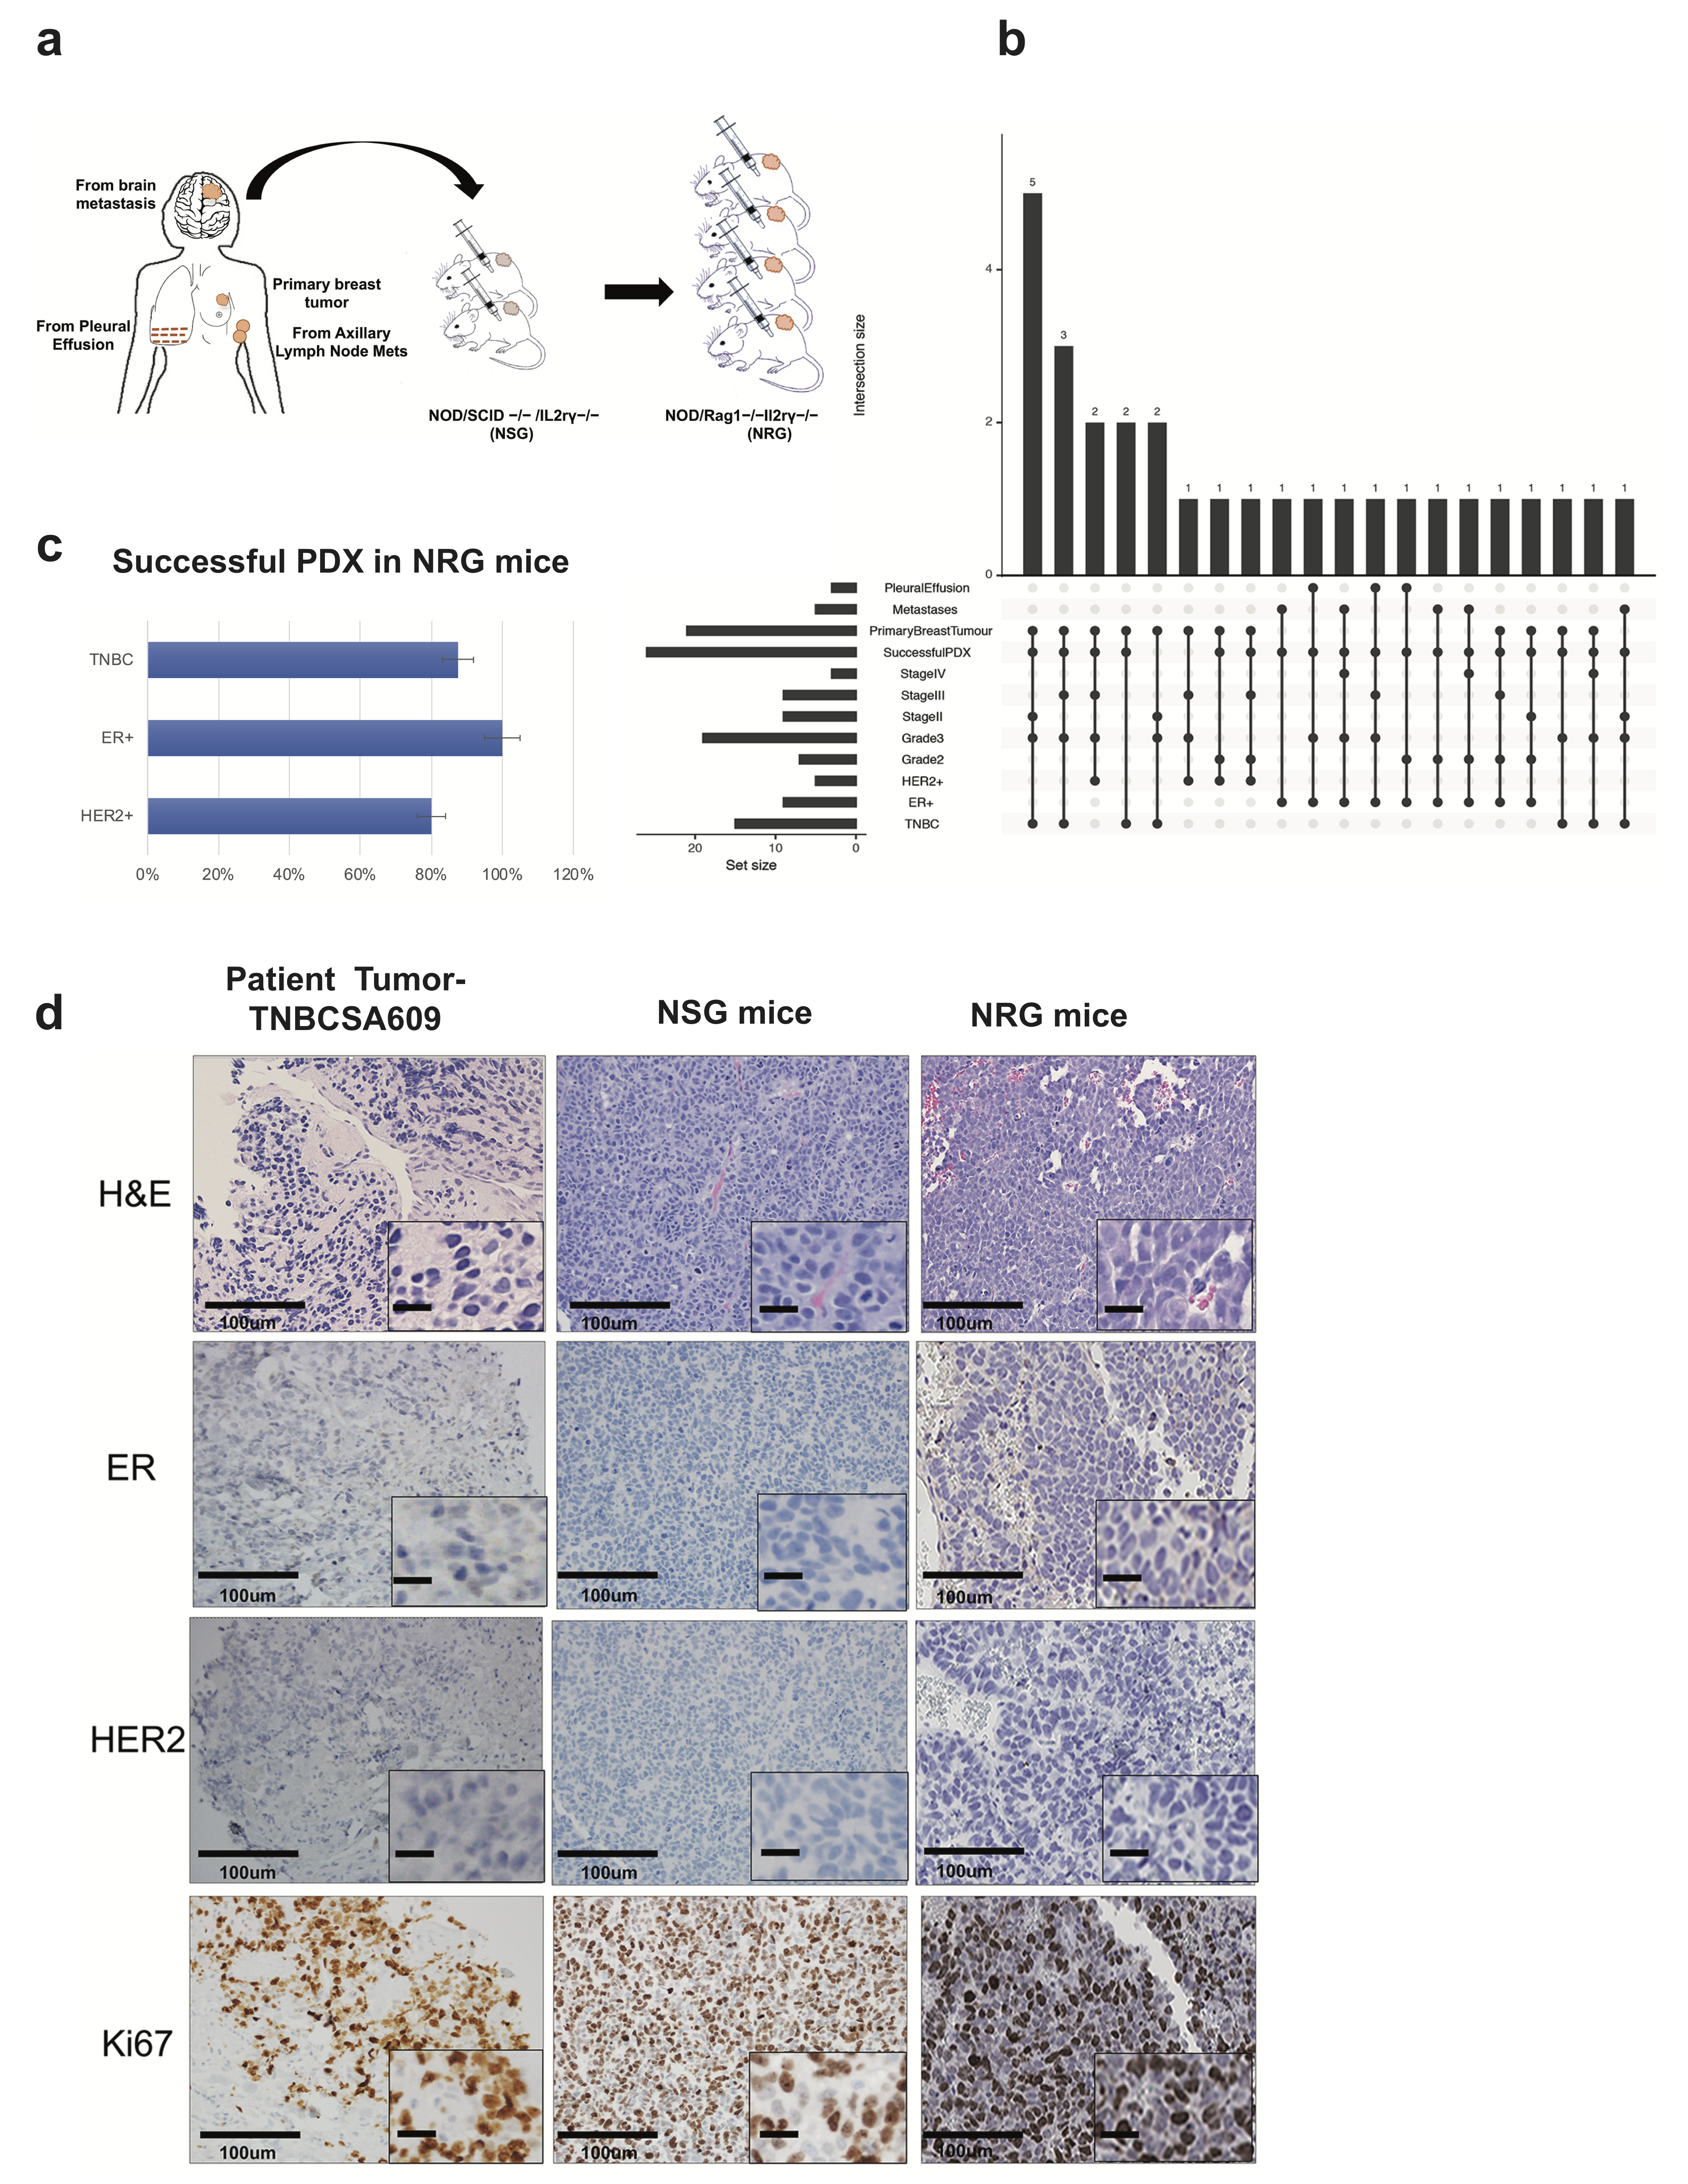
\includegraphics[width=\textwidth]{Figures/chap3/EstablishmentofPDX.png}
	\caption[Establishment of PDX in NRG mice]
	{\small
	    \textbf{Establishment of PDX in NRG mice.}
	    \textbf{(a)} Schematics of re transplant models in NRG.
	    \textbf{(b)} Venn sets bar plot of intersection sizes (upper panel) and group size bar plot (left panel). Vertical connectors below the intersection size bar plot show the corresponding set intersections.
	    \textbf{(c)} Summary of types of PDX and success rate.
	     \textbf{(d)} Representative histology images of TNBC-SA609. Red numbers on the upper right shows the stain scores.
	}

	\label{fig:EstablishmentofPDX}
\end{figure}

\subsubsection{Transplant rate in immunodeficient NOD Rag-1 null interleukin-2 receptor gamma null (NRG) mice remains high}
%Tumor samples were obtained from 30 breast cancer patients at BC cancer research centre from Vancouver, British Columbia hospitals and were implanted sub cutaneously into highly immunodeficient NOD/SCID/IL2r$\gamma^{\small{-/-}}$ (NSG) and NOD/Rag1$^{\small{-/-}}$Il2r$\gamma ^{\small{-/-}}$ (NRG)\cite{pearson2008non}. 

Breast cancer patient's tumour samples from primary tumour site, axillary lymph nodes, brain metastasis and pleural effusion were already established into highly immunodeficient NOD/SCID/IL2r$\gamma^{\small{-/-}}$ (NSG) in the lab \cite{eirew2015dynamics}. 
To set up and evaluate transplant models with drugs, I transplanted 29 of the established NSG tumours into NOD/Rag1$^{\small{-/-}}$Il2r$\gamma ^{\small{-/-}}$ (NRG) \cite{pearson2008non} \textbf{(\autoref{fig:EstablishmentofPDX} a, see methods)}.
Of the 29 implanted samples into NRG, 26 successfully established PDX tumours NRG mice (overall engraftment rate, 90\%). NSG IL2r$\gamma^{\small{-/-}}$ and NRG IL2r$\gamma^{\small{-/-}}$ are equivalent in immune deficiency functions, but NRG are more tolerant of DNA damaging chemotherapy drugs that comparatively have better tolerance to chemotherapies. 
The success rates according to breast cancer subtype were 100\% for HR+/HER2-ve, 80\% for HR-ve/HER2+, and 87.5\% for triple-negative breast cancer (TNBC) \textbf{\autoref{fig:EstablishmentofPDX} c}. Source of engraft tissue which came from patient's surgical specimens or biopsy did not affect PDX engraftment, consistent with previous results \cite{ryu2019integrative}. 
%Summary venn sets bar plot of intersection sizes (upper panel) and group size bar plot (left panel) for groups of interest (pleural effusion sample, metastatic sample, primary/secondary tumour status, xenograft success, stage, grade and tumour genotype). Vertical connectors below the intersection size \textbf{\autoref{fig:EstablishmentofPDX} b}, bar plot show the corresponding set intersections. For example, 
All of the tumour samples derived from pleural effusions were ER+ cases and produced successful xenografts. Tumour samples from two triple negative cases and one HER2+ case failed the transfer between NSG and NRG hosts \textbf{\autoref{fig:EstablishmentofPDX} b}.


\subsubsection{Histologic characteristics of the NSG mice corresponds to the NRG mice}

To confirm that histological features of the patient's original tumour were stably retained in the xenograft, we conducted a comparative histological analysis of xenograft tumours and tumours of origin using H\&E, ER, HER2 and Ki67 as biomarkers. 
\textbf{\autoref{fig:EstablishmentofPDX} d}, depicts histological results of representative patients and their xenograft tumours. For each subtype, morphological characteristics were conserved and hormone receptors, ER, HER2 along with Ki67 statuses were maintained throughout the respective xenografts. ER, PR and HER2 remained negative from NSG to NRG \textbf{(\autoref{fig:EstablishmentofPDX} d)}. 
Of the other tumour markers tested (EGFR, CK5/6, SMA, Vimentin, E-Cadherin, CK8 and CK14), a range of immunopositivity was found that was maintained between transplants. The range of score varies from negative (0) to 3+ in each independent tumour for each marker but the scores were consistent between NSG and NRG PDX tumours of same type as shown in representative histological images of TNBC-SA609 \textbf{(\autoref{fig:EstablishmentofPDX} d)}.


 The above results confirmed that PDX tumours in \ac{NRG} could be confidently used for downstream experiments as the main histological markers of the original tumours were conserved. Also, the PDX models of breast cancer developed in this study reflected the characteristics of the original tumours because Eirew et al. showed that comparisons of clonal dynamics by serial engraftment and propagation in NSG mice vs NRG mice suggested no major differences \cite{eirew2015dynamics}.

%---------------------------------------------------------------


\subsection{Short term \textit {in vitro} cultures reveals differential drug efficacy and PDX tissue responses
}
Next, we sought to establish drug efficacy of conventional chemotherapies and G4 quadruplex, CX-5461, to determine the broad range of the PDX tumour responses in short term \textit{in vitro} assays. The purpose of these experiments is to judge the dynamics of responses from various PDX tumors by using percent viability information along with the differences in their IC50 values across various tumour types. 
%It was essential to check the effectiveness of drugs across PDX tumors, in terms of therapeutic effectiveness before starting \textit{in vivo} screening, because, we intended to use patient's original clinical chemotherapies from pharmacy, where possible, instead of the drugs used for lab research only. 
The aim was to select at least 4 drugs for downstream \textit{in vivo} screening.

\subsubsection{Standard chemotherapies exhibit wide dynamics responses across various PDX in short term PDX cultures}

To evaluate the spectrum of drug sensitivity in short term PDX,
total of 7 PDX tumours, including 3 TNBC, 2 ER+ and 2 HER2+, were enzymatically digested into single cells and plated in 96-wells, collagen coated plates \textbf{\autoref{fig:invitro} a, see methods}. 
Briefly, PDX cells were incubated with various chemotherapies at 5 different concentrations after 24 hours of cell seeding. The dose sensitivities (7 days in drug) were quantified by using a WST-1 metabolic, cell viability assay (n=4). 

Notably, dose response inhibition curves \textbf{\autoref{fig:invitro} b} and estimated IC50 values from sigmoid fit \textbf{\autoref{tab:invitroIC50}}, showed that platinums (cisplatin, carboplatin), Taxanes (Paclitaxel, Docetaxel) and doxorubicin displayed wide dynamic range of -9(logIC50)M to -5(logIC50)M across multiple PDX. Moreover, CX-5461 showed a range of -9(logIC50)M to -6(logIC50)M \textbf{\autoref{fig:invitro} b}. In addition, 5 PDX cultures were exposed to PARP inhibitor, however, only TNBC-SA535, which was BRCA 1 deficient PDX, exhibited sensitivity to PARP inhibitor with -8(logIC50)M. 
BMH-21, Fluorouracil, Pyridostatin and Methotrexate were not very effective because of high IC50 values (minimum of -7(logIC50)M ) \textbf{(Summary results in \autoref{tab:invitroIC50}, representative response curves in \autoref{fig:invitro} a}. A new compound of our interest, CX-5461 also showed up with high efficacy and wide range of responses with very low IC50 values across different PDX tissues \textbf{\autoref{fig:invitro} b}. 

%\subsubsection{CX-5461 show higher drug sensitivity in LIG4$-$/$-$ and PRKDC$-$/$-$ HCT116 cells than wild type}

%To further explore the efficacy of CX-5461 and also to supplement another ongoing project in the lab, human colon cancer cell line (HCT116) wild type (WT) and LIG4$-$/$-$ and PRKDC$-$/$-$ were exposed to CX-5461 with same dose concentrations as in PDX (n=$>$4). PRKDC and LIG4 are key components of the \ac{NHEJ} pathway in mammalian cells \cite{drouet2005dna}. 
%The compelling findings was the differential response of CX-5461 with deficient DNA repair pathways \textbf{\autoref{fig:invitro} c}. The IC50 differences for CX-5461 between knock outs (LIG4$-$/$-$, PRKDC$-$/$-$) and their WT cells were around 5.73 (P$<$0.005, t-test) \textbf{\autoref{fig:invitro} c}. 
%These mechanisms were later explored in detail in the lab and was published by Xu \textit{et al}, \cite{xu2017cx}. 

Based on IC50 values and wide range of tumour responses,  CX-5461, cisplatin, paclitaxel and PARP inhibitors were selected for \textit{in vivo} screening.

%-------------------------------------------
\begin{figure}
	\centering
	\includegraphics[width=\textwidth]{Figures/chap3/invitro.png}
	\caption[Representative graphs from drug efficacy testing \textit{in vitro} ]
	{\small
	    \textbf{Drug efficacy testing \textit{in vitro}.}
	    \textbf{(a)} Schematics of experimental design
	    \textbf{(b)} Response of PDX tumour cells to chemotherapies \textit{in vitro} (n=4). Each graph represent each type of PDX tumour tested with the drugs mentioned in its key. Vertical axis represents percent viability normalized to control. Horizontal axis present drug doses.
	   
	}
	\label{fig:invitro}
\end{figure}

%-----------------------------------------------------------------

 % Table generated by Excel2LaTeX from sheet 'Sheet1'
 \begin{table}[htbp]
   \centering
   \caption{Summary of logIC50 values of PDX responses \textit{in vitro}}
     \begin{tabular}{|c|p{5em}|c|c|c|c|c|r|r|}
        \hline
       & \multicolumn{7}{|c|}{\textbf{Patient derived xenografts}} \\
          \hline
       & \textbf{SA429} & \textbf{SA500} & \textbf{SA501} & \textbf{SA532} & \textbf{SA535} & \multicolumn{1}{|c|}{\textbf{SA684}} & \multicolumn{1}{|c|}{\textbf{SA993}}\\
     \multicolumn{1}{|l|}{\textbf{Drug (LogIC50)M}} & \textbf{(ER+)} & \textbf{(HER2+)} & \textbf{(TNBC)} & \textbf{(HER2+)} & \textbf{(TNBC-HRD)} & \multicolumn{1}{|c|}{\textbf{(ER+)}} & \multicolumn{1}{|c|}{\textbf{(TNBC)}} \\
        \hline
     CX-5461  & -8.149 & -9.345 & -7.607 & -7.058 & -9.876 & -6.403 & -7.316 \\
     Cisplatin  & -7.28 & -6.324 & -7.680 & -6.302 & -6.987 & -6.08 & -5.954 \\
     Paclitaxel  & -6.965 & -6.48 & -9.6 & -7.519 & -8.324 & -6.338 & -9.274 \\
     Doxorubicin  & -9.122 & -7.238 & -9.361 & -7.498 & -7.2 & -7.014 & -8.951 \\
     BMH-21  & -5.866 & -6.932 & -6.527 & -5.502 & -7.281 & -6.508 & -5.951 \\
     Pyridostatin & -6.302 & N/A & N/A & N/A & -6.698 & -6.687 & -6.321 \\
     PARP inhibitor  & N/A & -6.208 & N/A & -5.894 & -8.348 & -7.798 & -6.484 \\
     Docetaxel  & N/A & -6.202 & -12.88 & N/A & -8.175 & -5.718 & -8.674 \\
     Fluorouracil (5-FU)  & N/A & -6.467 & -5.999 & N/A & -6.374 & -6.664 & -6.357 \\
     Carboplatin  & N/A & -5.946 & N/A & N/A & -6.373 & -6.583 & -6.009 \\
     Methotrexate  & N/A & -7.576 & -7.203 & N/A & -7.589 & -6.088 & -7.794 \\
    
     \hline
     \end{tabular}%
   \label{tab:invitroIC50}%
   
   
    \small\textbf{ (N/A means not measured)}.
 \end{table}%

%%%%%%%%%%%%%%%%%%%%%%%%%%%%%%%%%%%%%%%%%%%
\begin{figure}
\centering
	\includegraphics[width=\textwidth]{Figures/chap3/4drugs4PDXnew.png}
	\caption[Representative tumour responses from four PDX and  to four drugs]
	{\small
	   \textbf{Representative tumour responses from four PDX and  to four drugs.}
	    \textbf{(a)} Tumour growth curves from treated and un treated tumours. Vertical axis-left, represents the tumour volume in cubic millimeters; vertical axis-right, represents the drug and treatment status. Horizontal axis represents the days post-measurable tumours. Red arrows represent the time of start of treatments,
	   \textbf{(b)} Bar plot showing tumour growth inhibition percentages. Error bars represent 95\% bootstrap confidence interval based on 2-4 replicates.  \textbf{(c)} Response summary matrix of \textbf{a} based on quantified tumour growth inhibition in \textbf{b}.
	    }
	\label{fig:invivo}
\end{figure}

%%%%%%%%%%%%%%%%%%%%%%%%%%%%%%%%%%%%%%%%%%%


% Table generated by Excel2LaTeX from sheet 'table for R'
\begin{table}[htbp]
  \centering
  \caption{Summary responses \textit{in vivo} with 3x1x1 strategy trichotomized tumour response based on TGI \cite{hather2014growth, aykan2020objective}}
    \begin{tabular}{|l|l|l|l|l|}
    
     \hline
    \textbf{Tumour ID} & \textbf{Cisplatin} & \textbf{Paclitaxel} & \textbf{Rucaparib} & \textbf{CX-5461} \\
     \hline
    HER2+SA532 & N/A   & N/A   & N/A   & Sensitive \\
    TNBC-SA535 & Sensitive & Sensitive & Partially-Sensitive & Sensitive \\
    TNBC-SA605 & Sensitive & Sensitive & N/A   & N/A \\
    TNBC-SA604 & Sensitive & Sensitive & Resistant & Resistant \\
    TNBC-SA609 & Sensitive & Sensitive & Resistant & Resistant \\
    TNBC-SA919 & N/A   & Sensitive & N/A   & N/A \\
    HER2-SA920 & N/A   & N/A   & N/A   & Resistant \\
    TNBC-SA993 & N/A   & N/A   & N/A   & Sensitive \\
    ER+SA995 & N/A   & N/A   & N/A   & Partially-Sensitive \\
    TNBC-SA1035 & Sensitive & Partially-Sensitive & Resistant & Sensitive \\
    TNBC-SA1130 & Sensitive & N/A   & N/A   & Sensitive \\
    TNBC-X2371 & Sensitive & Partially-Sensitive & N/A   & Sensitive \\
    TNBC-X2440 & Sensitive & Sensitive & N/A   & N/A \\
     \hline
    \end{tabular}
   \label{tab:PDXtumorsinvivo}
 
 \small\textbf{PDX ID = Patient-derived xenograft identification, N/A means not measured}\\
 

   \small\textbf{ (Tumour growth inhibition (TGI): Sensitive= $>$60\%; Partially-Sensitive= $>$30\% but $<$60\%; Resistant= $<$30\%)}.
\end{table}%

%%%%%%%%%%%%%%%%%%%%%%%%%%%%%%%%%%%%%%%%%%%



%--------------------------------------------

\subsection{Baseline \textit{in vivo} sensitivity patterns of triple negative breast cancer}
To evaluate the spectrum of baseline sensitivity of PDX tumours with conventional and novel targeted chemotherapies, I modified previously published 1x1x1 design, for semi-quantitative PDX drug sensitivity mapping, by increasing the number of replicate mice to a 3x1x1 design. \cite{gao2015high, migliardi2012inhibition}. 
%We performed \textit{in vivo} screen to model inter-patient response heterogeneity with \textbf{three animals per model per treatment strategy (3x1x1)}. 
 13 PDX were tested with cisplatin, Paclitaxel, Rucaparib or CX5461. Notably, all 8 of the TNBC tested were sensitive to cisplatin with tumour growth inhibition of more than 60\%, however, less responsive to Rucaparib \textbf{Summary in \autoref{tab:PDXtumorsinvivo}}. 
I selected in total of four 
TNBC PDX, including: 
\\
\textbf{TNBC-SA609} (Basal, FBI)
\\
\textbf{TNBC-SA1035} (Basal, APOBEC-like, HRD-like- BRCA 1 germline)
\\
\textbf{TNBC-SA535} (Basal, BRCA1 deficient)
\\
\textbf{TNBC-SA604} (Basal, FBI)
\\
 The drugs, including, two standard chemotherapies, platinum (cisplatin-(2mg/kg, \ac{Q3Dx8}, \ac{IP} max)) and Taxanes (Paclitaxel-13mg/kg, \ac{Q3Dx8}, \ac{IP} max), and two targeted chemotherapies, PARP inhibitor (Rucaparib-\ac{IP} daily 5 days per week for 3 weeks) and G4 quadruplex stabilizer (CX-5461-50mg/kg, \ac{Q3Dx8} by oral gavage). 

%\textbf{\autoref{fig:invivo} a} showing summary matrix of four triple negative breast (TNBC) PDX towards chemotherapies. 
%The growth curves are shown in \textbf{\autoref{fig:invivo} c}, including 

%TNBC-SA609 (Basal, TP53, FBI), TNBC-SA1035 (Basal, APOBEC-like, POLH), TNBC-SA535 (Basal, MMRD-1, S-Dup, TP53, BRCA1 def) and TNBC-SA604 (Basal, CI-SV, CI-FBI).

To classify tumour responses, I measured tumour growth inhibition percent (TGI\%) in each PDX and divided them into three categories according to modified RECIST criteria \cite{aykan2020objective}. Sensitive: \ac{TGI} $>$60\%; partially sensitive: \ac{TGI} $>$30\% but $<$60\%; Resistant: \ac{TGI} $<$30\% \textbf{(\autoref{fig:invivo} a, c)}.
Not surprisingly, I found that all TNBC PDX with different background mutational signatures behaved differently towards the same drugs. Both PDX with FBI backgrounds, TNBC-SA609 and TNBC-SA604 were both found to be resistant to CX-5461 with tumour growth inhibition (TGI) of 15\% and 7\%, respectively \textbf{\autoref{fig:invivo} a, b}. Moreover, they were resistant to Rucaparib as well, with \ac{TGI} of 9\% and 16\%, respectively.
All four of the PDX showed high sensitivity to platinum (cisplatin). Three out of four PDX were sensitive to (taxane) paclitaxel, while TNBC-SA1035 (APOBEC, HRD-like) was partially sensitive with \ac{TGI} of 34\%. Surprisingly, TNBC-SA535 (BRCA 1 deficient), which was expected to be very sensitive to Rucaparib, showed growth inhibition of only 36\%  (partially sensitive) \textbf{\autoref{fig:invivo} c}.


\section{Optimization methods in tumour dissociation for single cell analysis}

This section of chapter 3 was published in \textit{Genome Biology, 2019} paper, title  \textbf{``Dissociation of solid tumour tissues with cold active protease for single-cell RNA-seq minimizes conserved collagenase-associated stress responses''}.
%%%%%%%%%%%%%%%%%%%%%%%%%%%%%%%%%%%%%%%%%%%%%%%%%%%%%%%%%%%%%%%%%%%%%%

\begin{figure}
	\centering
	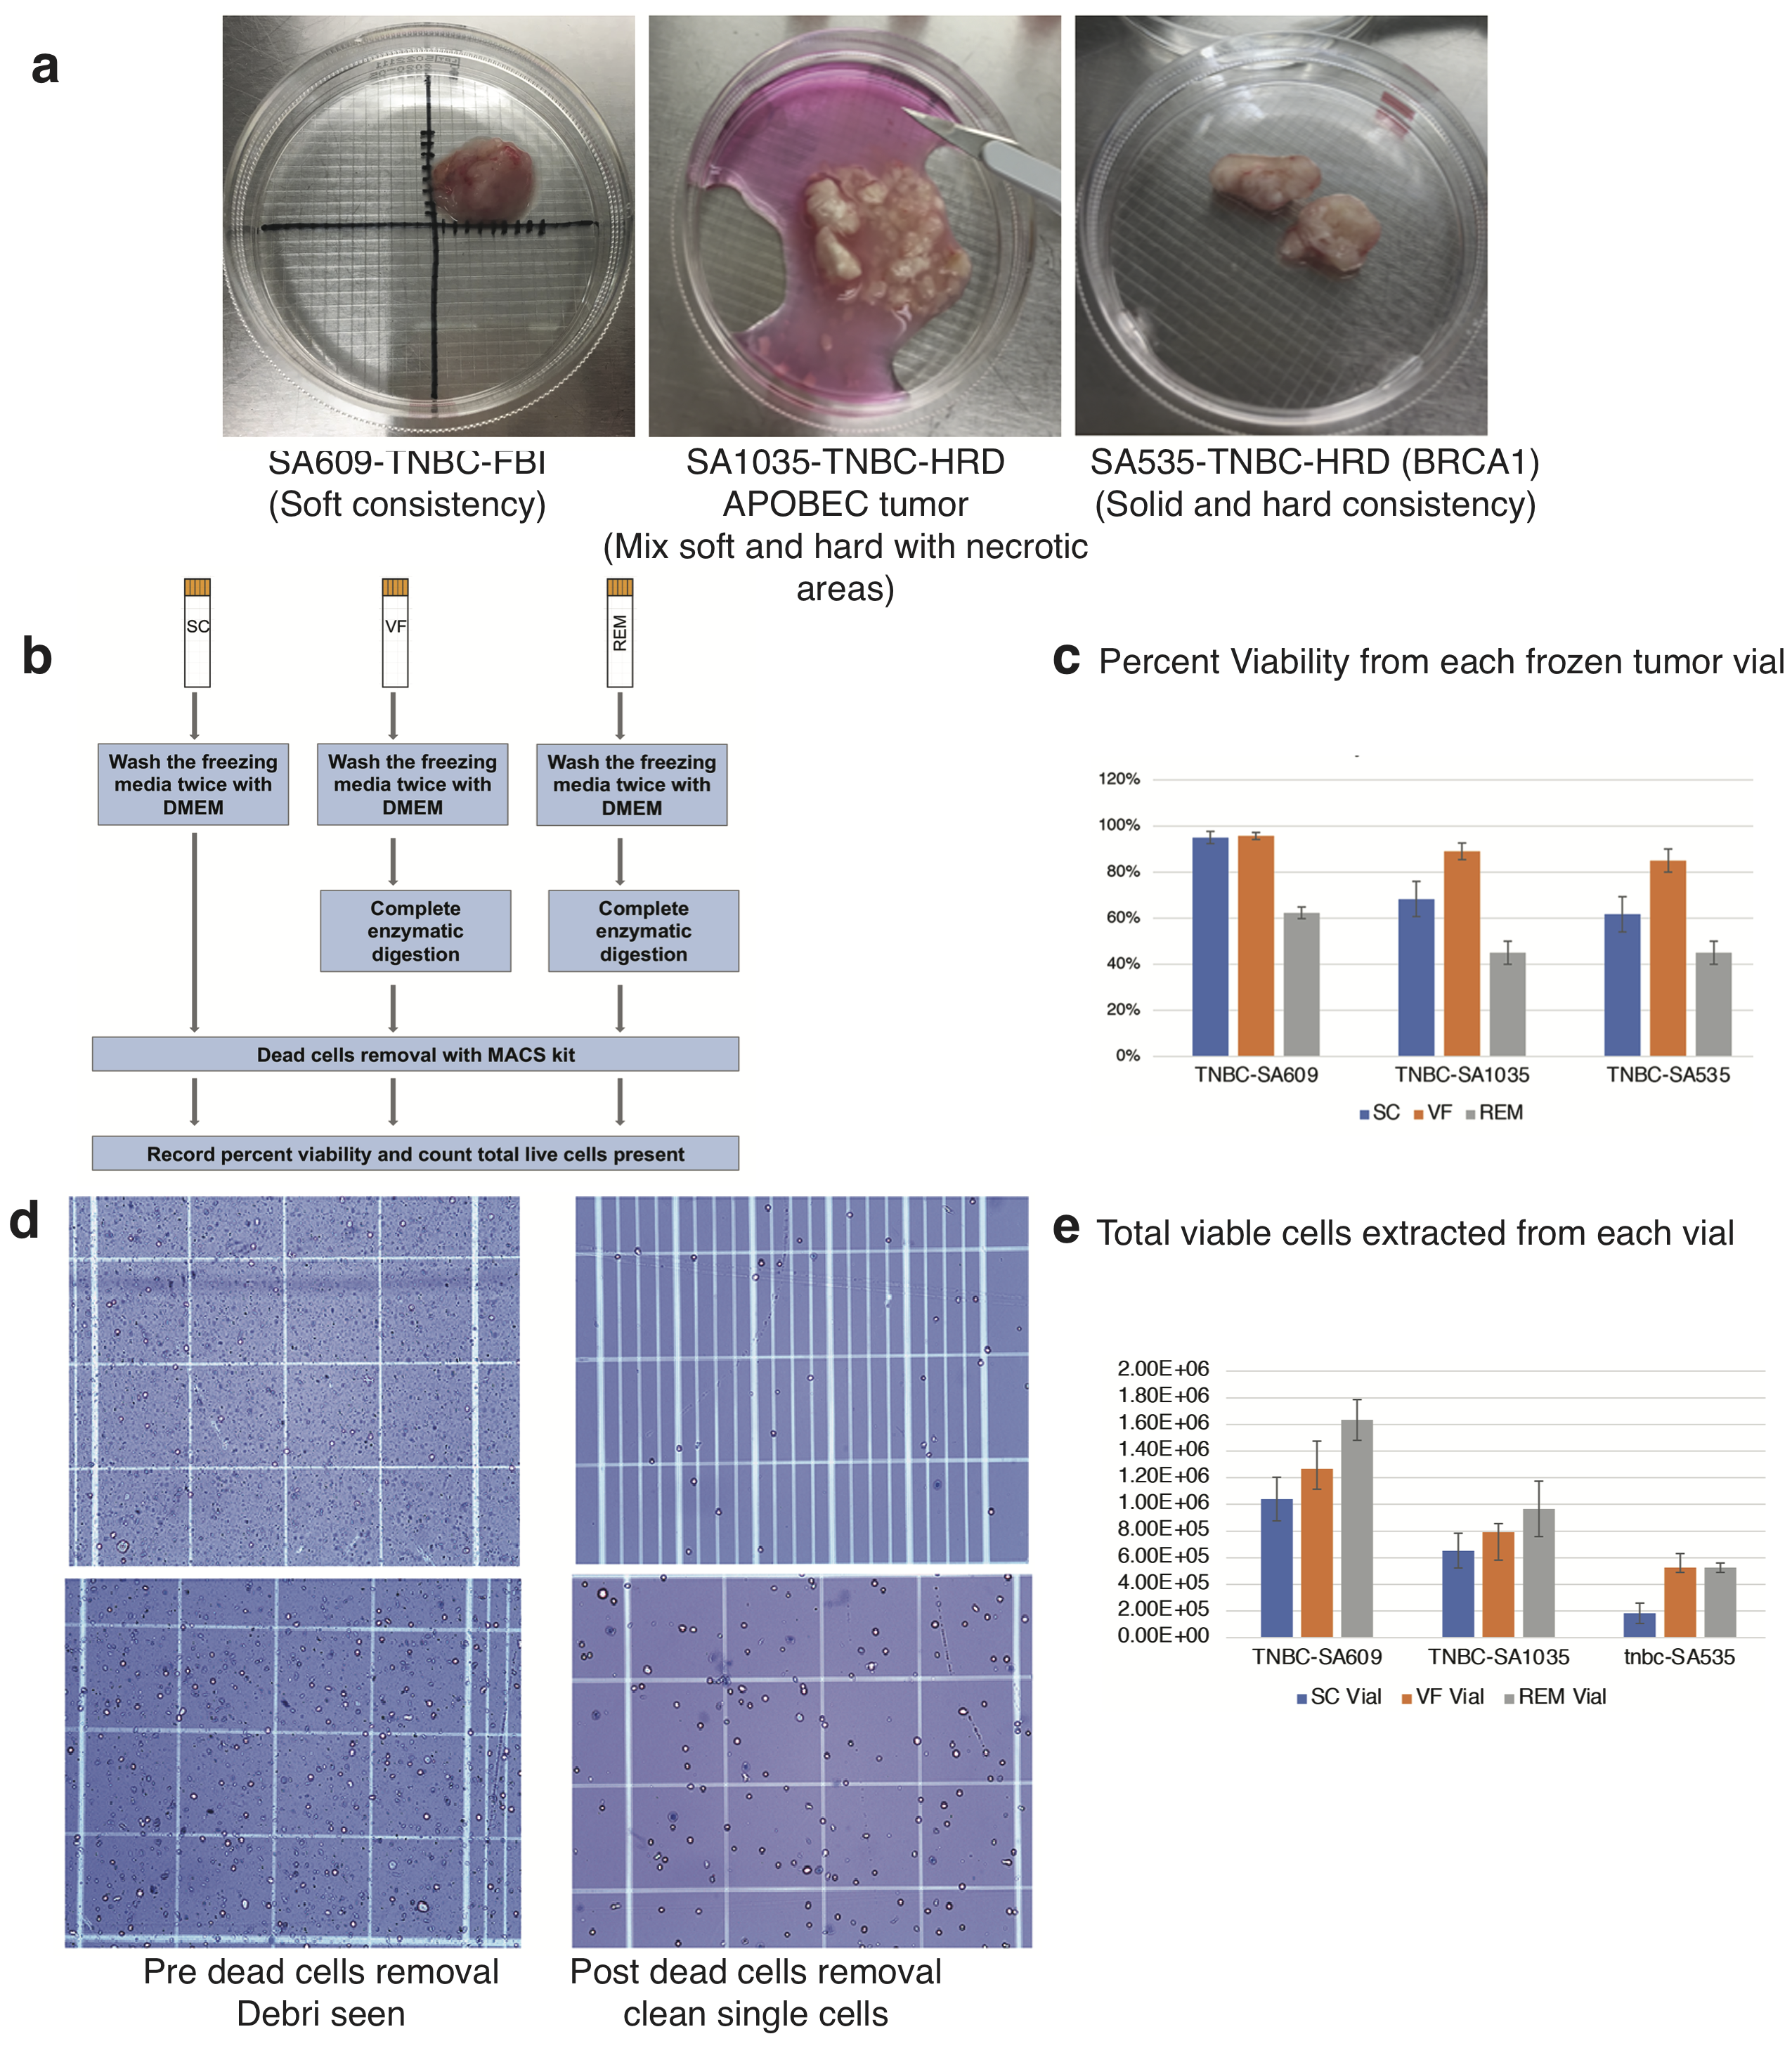
\includegraphics[width=\textwidth]{Figures/chap3/cellviability2.png}
	\caption[Evaluation of viable-high percent cell recovery for single cell measurements]
	{\small
	    \textbf{Evaluation of viable-high percent cell recovery for single cell measurements.}
	    \textbf{(a)} Representative tumours in dishes. Two small black lines as 2mm. Middle dish showing partially chopped tumour with white necrotic tissues. Right side panel showing example from comparatively solid to cut tumour.
	    \textbf{(b)} Schematics of processing of frozen vials. single cells (SC), Viable frozen (VF) and remaining big chunks (REM).
	    \textbf{(c)} Vertical axis showing the percent viability and horizontal axis: tumour type. Error bars represent one standard deviation from the mean. \textbf{(d)} Vertical axis: number of viable cells obtained from each vial and horizontal axis tumour type. Error bars: one standard deviation from the mean.\textbf{(e)} Left: pre-dead cell removal; right: post-dead removal on hemocytometer. \textbf{(f)} Vertical axid represent percent viability and   horizontal axis: tumour type. Error bars: one standard deviation from the mean.  
	}
	\label{fig:cellviability}
\end{figure}
%%%%%%%%%%%%%%%%%%%%%%%%%%%%%%%%%%%%%%%%%%%%%%%%%%%%%%%%%%%%%%%%%%%%%%


\subsection{Small viable frozen fragments of the tumours culminated in high viability and less debris as compared to big frozen chunks}
To investigate the method of tissue freezing that could provide optimal single cell suspensions for downstream analysis, I mechanically disaggregated (paddle blender, \cite{eirew2015dynamics}, also see methods) three TNBC PDX tumours \textbf{\autoref{fig:cellviability} a}, TNBC-SA609, TNBC-SA1035 and TNBC-SA535 and cryopreserved with three protocol variations. First, after mechanical digestion, small organoid-like cell clumps (VF) were cryopreserved in the freezing media. Second, full dissociation (with collagenase/Hyaluronidase) to single cell (SC) suspensions, third, remaining large tissue fragments (REM) were cryopreserved. 
Tumour fragments were thawed and washed twice with 
Gibco Dulbecco's Modified Eagle Medium (DMEM) media. VF and REM fragments were digested to single cells with collagenase hyaluronidase and dead cells and debris were removed from all the single cells final suspension as described in the method section \textbf{\autoref{fig:cellviability} b}. I obtained high proportion of viable cells from viable frozen (VF) tumour fragments across all the three tested PDX tumours ranging 82\% for REM fragment cryopreservation to 95\% for single cell suspensions (SC) \textbf{\autoref{fig:cellviability} c}.
However, the final number of viable cells in each of the condition across different PDX varies from 200 thousands to one million cells \textbf{\autoref{fig:cellviability} d}. Interestingly, High viability was obtained from SA609 in all conditions. 
It was concluded that across all conditions and PDX lines tested, VF organoid cryopreservation was the most consistent and was therefore chosen as the standard method for all subsequent experiments.

%Finally, in order to  remain consistent across every type of tumor, I  concluded that Viable frozen "VF" was the best option as providing  moderate number of viable cells across xenografts.
Finally, single cell suspension from all three PDX were tested for high proportion of viable cells pre or post dead cell removal step. First, cell viability was recorded before dead cell removal. Then, dead cells, debris and dying cells were eliminated by magnetic activated cell sorting (MACS) columns (Miltenyi Biotec, dead cell removal kit, according to manufacturer's protocol). Briefly, for the dead cell
depletion, cells were magnetically labeled with dead cell removal
microbeads, that recognize a moiety in the plasma
membrane of apoptotic as well as dead cells, and passed through a separation column. These columns were placed within the magnetic field. Apoptotic cells present in the single cell suspension would bind to the Annexin V containing microbeads and stayed in the column, while the effluent would contain live cells. It was found that single cell field on the hemocytometer was much cleaner after dead cells and debris removal \textbf{\autoref{fig:cellviability} e}.
The percentage of viable cells was increased from 69\% to 95\% in SA609, 54\% to 91\% in SA1035 and from 47\% to 88\% in SA535 PDX tumour cells \textbf{\autoref{fig:cellviability} f}. 




%----------------------------------------------------------------


%--------------------------------------------------------------------

\subsection{Dissociation with Collagenase at 37\textdegree C induces a distinct stress response in single-cell transcriptomes}
To uncover transcriptional variation and responses to dissociation method and to see the effect of digestion temperature on the transcriptome, I generated scRNA-seq data from a range of PDX tumours dissociated at low temperature with cold active protease and at high temperature with collagenase and Hyaluronidase, using the 10x Genomics Chromium v3 platform \textbf{(see methods)}.
We performed a differential expression analysis on the 23,731 cells found by combining all experiments measured in PDX tumours at either 6\textdegree C or 37\textdegree C. After retaining genes with at least 10 counts across all cells, we performed differential expression analysis with edgeR \cite{robinson2010edger}, while controlling for the sample-of-origin.
We found that of the 19,464 genes retained for analysis, 11,975 (62\%) were differentially expressed at a Benjamini-Hochberg corrected false discovery rate (FDR) of 5\%. We defined a core set of genes meaningfully perturbed by digestion temperature as those significantly differentially expressed as above, but with an absolute log fold change of at least 1.5. Therefore, for a gene to be included under these criteria it must be differentially expressed and its abundance increased or decreased by at least 50\% by digestion temperature. 

%-------------------------------------------------------------------------

\begin{figure}
	\centering
	\includegraphics[width=\textwidth]{Figures/chap3/stressresponse1.png}
	\caption[Dissociation with collagenase induces a distinct stress response in PDX tumours]
	{\small
	    \textbf{Dissociation with collagenase induces a distinct stress response in PDX tumours.}
	    \textbf{(a)} The top 40 genes (by log fold-change) from the 11,975 identified as significantly differentially expressed between cells digested at 6\textdegree C and 37\textdegree C.
	    \textbf{(b)} UMAP plots of 23,731 cells coloured by digestion temperature (top) then by normalized expression of 3 key stress response genes (\textit{FOS}, \textit{JUNB}, \textit{NR4A1}) demonstrates a distinct concordance between temperature and induction of the stress gene signature.
    Expression values are log normalized counts winsorized to $[0,2)$ then scaled to $[0,1)$
	    \textbf{(c)} Pathway analysis of differentially expressed genes with the MSigDB hallmark gene sets highlights induction of genes involved in NF-$\kappa$B signalling at 37\textdegree C digestion with 46.5\% of 200 genes annotated in the pathway being found in the 512 core gene set}
	\label{fig:stressresponseinpdx}
\end{figure}

%-------------------------------------------------------------------------

This produced a core gene set of 512 genes, of which 507 were upregulated at 37\textdegree C and the remaining 5 downregulated. This gene set included multiple canonical stress-related genes such as \textit{FOS}, \textit{FOSB}, \textit{ATF3} and heat shock proteins (HSPs) \textbf{\autoref{fig:stressresponseinpdx} a}, expression of which had shown to be induced by collagenase dissociation in a subset of muscle cells \cite{van2017single}. A \ac{UMAP} embedding of the cells coloured by dissociation temperature and the expression of several key genes (\textit{FOS}, \textit{JUNB}, \textit{NR4A1}) \textbf{\autoref{fig:stressresponseinpdx} b}, further demonstrated the digestion temperature-specific induction of the expression of these genes.
We subsequently performed a pathway enrichment analysis on the differential expression results, searching for enrichment in given hallmark pathways \cite{liberzon2015molecular} \textbf{\autoref{fig:stressresponseinpdx} c}. Of particular note was TNF (tumour necrosis factor) signalling via NF-$\kappa$B of which 46.5\% of annotated pathway genes were included in the core set of 512 genes. Further enrichment of stress-associated pathways including hypoxia, apoptosis, and inflammatory response was further indicative of collagenase dissociation at 37\textdegree C as inducing a stress response on the transcriptomes of single cells.

 \subsection{Identification of subpopulations of dead, dying and live cells in transcriptomic data}
Given the bi- and tri-modal distributions of mitochondrial gene count percentages \cite{o2019dissociation} apparent in the PDX experiments and previous studies' assertions that high mitochondrial gene content is indicative of dead and dying cells \cite{ilicic2016classification, zhao2002mitochondrial}, we next sought to determine the contribution of dead and dying cells to the variation observed in QC metrics  \cite{o2019dissociation}. In order to induce classical cell death pathways, we used TNF\textalpha    
  \cite{carswell1975endotoxin, sedger2014tnf} to treat the non tumourigenic, lymphoblastoid cell line GM18507 and FACS sorted cells into dead or and dying fractions based on PI/Annexin V positivity \textbf{\autoref{fig:livedead} a)}, as well as a live, untreated fraction. Notably, cell yield from scRNAseq data was highly dependent on the cell status, with 8,597 live cells recovered but only 1,280 and 885 dead and dying, respectively, compared to targeted numbers of 3,000 cells. 
A principal components analysis (PCA) following mutual nearest neighbours (MNN) correction \cite{haghverdi2018batch} demonstrated the cells approximately segregating along the first principal component (PC1) by cell status \textbf{\autoref{fig:livedead} b)}, albeit with high levels of heterogeneity in overlap. Indeed, PC1 closely tracked the mitochondrial gene content of the cells \textbf{\autoref{fig:livedead} c)}, being significantly higher in dead cells (median 29.9\%) compared to both dying cells (median 3.13\%, $p=1.17 \mathrm{e}{-126}$) and live cells (median 3.4\%, $p=4.65 \mathrm{e}{-153}$) as shown in \textbf{\autoref{fig:livedead} d}.
This observation justifies the practice of excluding cells with very high mitochondrial gene content as being likely dead cells.

Conscious of the possibility of murine stromal cell contamination in PDX samples, we classified cells as mouse or human based on alignment metrics. Of the 99,244 PDX cells sequenced, 4942 were reliably identified as mouse cells, with large inter-sample variation \textbf{\autoref{fig:mouseqc}}.
As expected, murine cells scored consistently lower across a range of standard QC metrics (percentage of mitochondrial counts, total genes detected, total \ac{UMIs} detected) when aligned to the human genome \textbf{(see methods)}.
%-----------------------------------------------------------

\begin{figure}
\centering
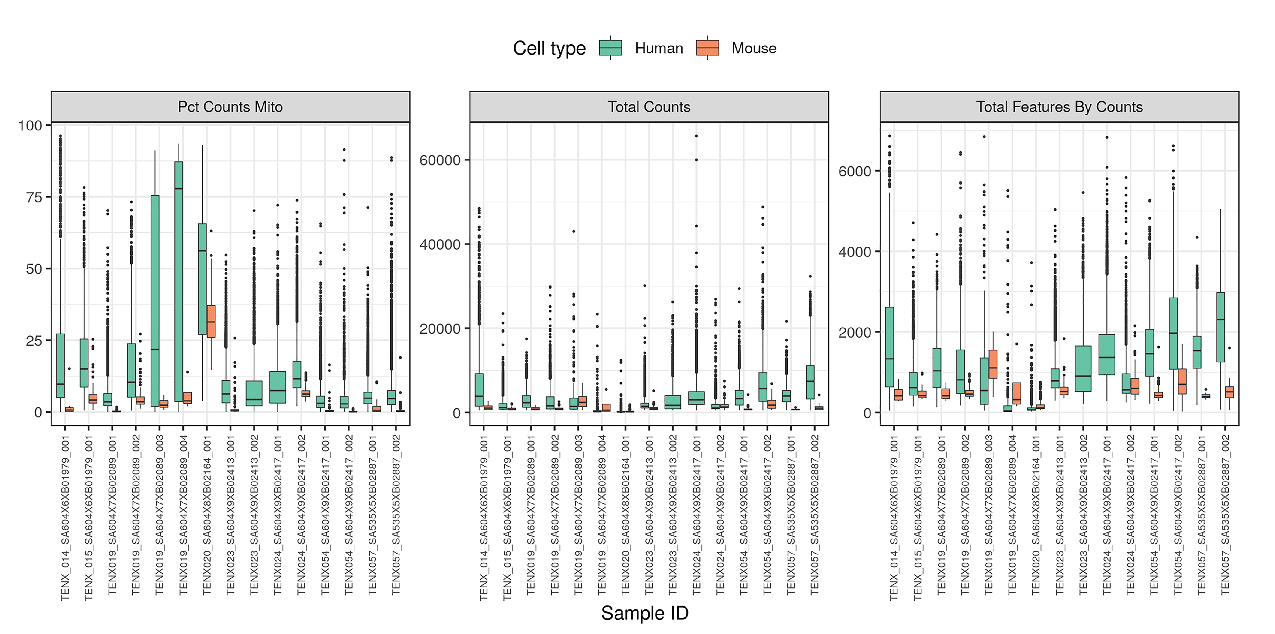
\includegraphics[width=\textwidth]{Figures/chap3/mouseqc.png}
	
\caption[Quality control metrics (\% mitochondrial gene counts, total counts, total genes detected)]
	{\small
	\textbf{Quality control metrics (\% mitochondrial gene counts, total genes detected).}
	 All scRNA-seq of PDX included in the study, on average, of murine cells score lower across all three metrics though with notable inter-dataset variability.
	   \textbf{(a)} Vertical axis represents the percentage of mitochondrial genes detected in mouse or human samples. Horizontal axis denotes the sample IDs from each of the PDX library. 
	  \textbf{(b)} Vertical axis represents the total features (genes) of  genes detected in mouse or human samples. Horizontal axis denotes the sample IDs from each of the PDX library. 
	}
	\label{fig:mouseqc}
\end{figure}

%-----------------------------------------------------------------------
\begin{figure}
	\centering
	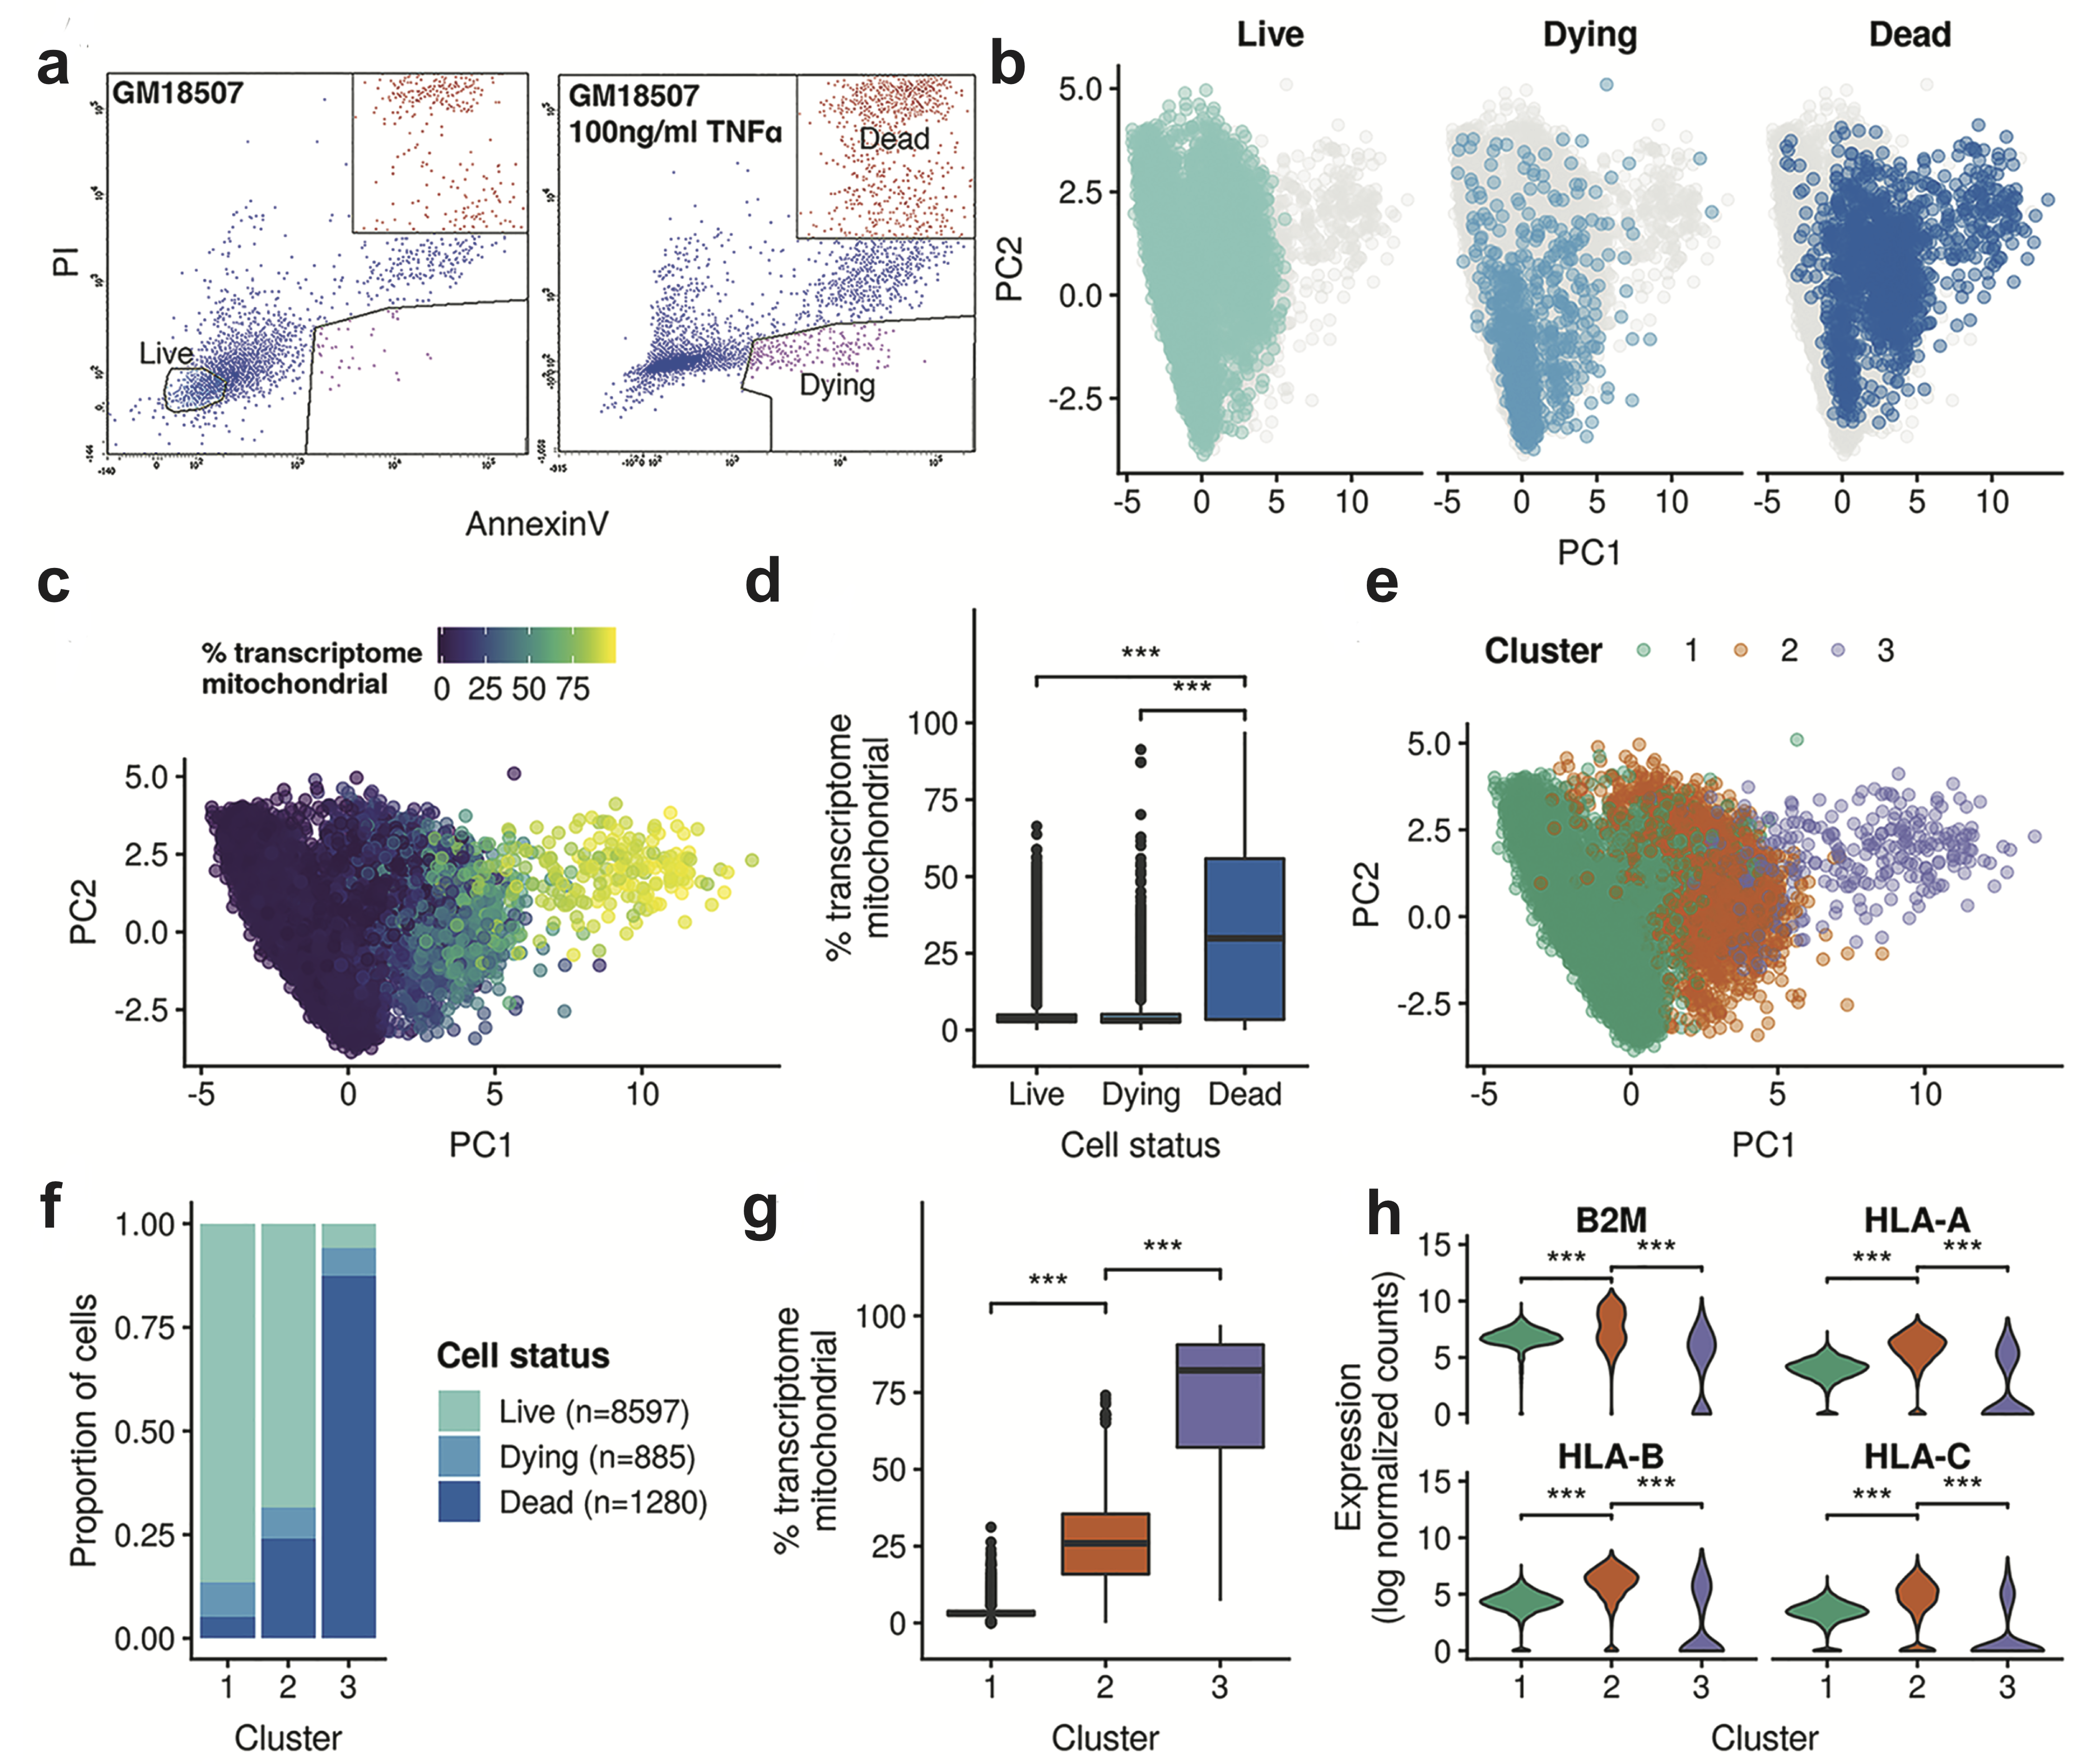
\includegraphics[width=\textwidth]{Figures/chap3/livedead.png}
	\caption[Transcriptomic landscape of live, dead, and dying cells.]
	{\small
	    \textbf{Transcriptomic landscape of live, dead, and dying cells.}
	    \textbf{(a)} FACS analysis showing gating strategy for untreated, live cells (PI$-$/annexin V$-$) or TNF\textalpha-treated dying cells (PI/annexin V+) and dead cells (PI+/annexin V+).
	    \textbf{(b)} PCA projection of the three cell conditions showing approximate segregation of cell status along the first principal component (PC1), with live and dying cells enriched at lower PC1 values and dead cells enriched at higher values.
	    \textbf{(c)} PCA projection colored by the percentage mitochondrial genes (``\% transcriptome mitochondrial'') shows significant increase along the PC1 \textbf{(d)} Dead cells exhibit significantly higher percentage of the transcriptome as mitochondrial compared to both live and dying cells \textbf{(e)} Unsupervised clustering of the gene expression profiles clusters the cells into three groups, approximately tracking both PC1 of the data and the percentage of transcriptome mitochondrial \textbf{(f)} The composition of each cluster demonstrates that cluster 1 is primarily composed of live cells, cluster 2 a mix of live, dying, and dead cells, while cluster 3 is composed mainly of dead cells \textbf{(g)} The\% transcripts mitochondrial is significantly different between the three clusters, with a step increase in proportion moving from cluster 1 to 2 and 2 to 3 \textbf{(h)} Cluster 2 significantly up-regulates the MHC class I gene set, suggesting it represents stressed or pre-apoptotic cells.
	}
	\label{fig:livedead}
\end{figure}

%-------------------------------------------------------------------------

\begin{figure}
	\centering
	\includegraphics[width=\textwidth]{Figures/chap3/livedead2.png}
	\caption[Differential expression of cluster 1 of live, dead, and dying cells.]
	{\small
	 \textbf{Differential expression of cluster 1 of live, dead, and dying cells.}
    \textbf{a} Differential expression analysis of transcriptomically ``healthy'' cells within cluster 1 reveals residual differences between cells sorted as live and dead.
    \textbf{b} The distribution of absolute effect sizes (log fold change) of live vs. dead cells within cluster 1 (x-axis) compared to between clusters 1 and 2 (y-axis) demonstrates the residual effect on the transcriptome of being live/dead sorted is small compared to the inter-cluster expression variance.}
	\label{fig:livedead2}

\end{figure}
%-----------------------------------------------------------

Having observed that the transcriptomes of the different cell conditions are not entirely distinct, we sought to discover the extent of mixing between transcriptomic states and whether live and dead cells that appear transcriptomically ``healthy'' (i.e would ordinarily pass QC) are distinguishable. Using hierarchical clustering \textbf{(see methods)}, we clustered the cells into 3 groups  that approximately track PC1  \textbf{\autoref{fig:livedead} e)}. Interestingly, these three groups show variable composition in terms of cell states, with cluster 1 being comprised mainly of live cells (86\% live, 8.5\% dying, 5.1\% dead), cluster 2 containing an increased proportion of dying and dead cells (68\% live, 7.5\% dying, 24\% dead), and cluster 3 comprised mainly of dead cells (5.9\% live, 6.7\% dying, 87\% dead). This clearly demonstrates that cluster 1 is primarily composed of live cells and cluster 2 a mix of live, dying, and dead cells, while cluster 3 is composed mainly of dead cells, \textbf{\autoref{fig:livedead} f)}. Furthermore, we observed a step change increase in mitochondrial gene content between clusters \textbf{\autoref{fig:livedead} g)}, with cluster 1 having the lowest (median 3.13\%), followed by cluster 2 having a significant increase (median  26\%, $p=$ 0) and cluster 3 having a significant increase beyond that (median 82.2\%, $p=2.35\mathrm{e}{-149}$). 

Differential expression analysis between these clusters revealed a significant up-regulation in stress-associated pathways such as MHC class I,  \textbf{\autoref{fig:livedead} h)} in cluster 2 compared to clusters 1 \& 3. MHC class I genes are involved in antigen presentation to T cells, but are also expressed in many cell types and are induced in response to stress stimuli and contain heat shock-inducible elements \cite{gleimer2003stress}. 

Together, these results suggest a model whereby cluster 1 represents transcriptomically ``healthy'' cells, cluster 2 represents transcriptomically stressed cells that upregulate stress pathways  and have increased mitochondrial gene content (due to either an increasingly permeable membrane causing loss of cytoplasmic mRNA or increased metabolic demands), and cluster 3 represents transcriptomically dead cells whereby the membrane has burst leaving majority mitochondrial transcripts. Importantly, cells that are FACS sorted as either live, dying, or dead, are present in all three clusters, highlighting that the transcriptomic state of the cell is not necessarily the same as the surface marker state (though the two are correlated). Such concepts are reminiscent of ``pseudotime'' in single-cell developmental biology, whereby developmentally ordering cells transcriptomically can lead to early or late cells being placed at variable positions along the pseudotime trajectory \cite{campbell2018descriptive,campbell2018uncovering}. Indeed, PC1 from \textbf{\autoref{fig:livedead} a} approximates a pseudotime trajectory through the data, that tracks transcriptomically healthy cells to transcriptomically dead cells with increasing PC1 values.

\subsection{Live sorted and dead cells exhibit gene expression differences}
Next, we sought to determine if a sorted dead cell that appears transcriptomically healthy remains distinguishable from a sorted live cell in the transcriptomically healthy group. Using only cells in cluster 1, we further subsetted them to pass a strict set of QC filters (at least $10^3$ total genes detectable, \% mitochondrial content between 1 and 10) and performed a differential expression analysis between cells sorted as live and dead in this group. Of the 10,537 genes retained for analysis, 2,130 (20.2\%) were found to be differentially expressed \textbf{\autoref{fig:livedead2} a}, including downregulation of \textit{IFITM1} in dead cells. To compare this type of variation to the inter-cluster transcriptomic variation, we performed a second differential expression analysis between clusters 1 and 2, finding 8835 of 10,933 (80.8\%) genes significantly differentially expressed. Furthermore, the effect sizes were significantly larger for the inter-cluster comparison than the within-cluster 1 live-dead comparison as demonstrated by the quantile-quantile plot of absolute effect sizes in the \textbf{\autoref{fig:livedead2} b}. Collectively, these results suggest that though there are gene expression differences between dead and live sorted cells within cluster 1, the magnitude of expression variation is small compared to transcriptomically stressed clusters.
 
\subsection{Transcriptomic stress response is induced by both digestion time and digestion temperature}
To determine whether the gene signature identified above was induced due to the longer digestion time required for complete collagenase dissociation or due to the enzyme itself, we conducted a time course experiment, incubating breast PDX tissue with collagenase or cold protease for up to 3 hours. Since proteases work at different speeds on intact tissues, single cells released into the supernatant were sampled at 30 minutes, 1 hour, 2 hours or 3 hours.   

%------------------------------------------------------------------------- 

\begin{figure}
	\centering
	\includegraphics[width=\textwidth]{Figures/chap3/digestiontime.png}
	\caption[Differential expression of cluster 1 of live, dead, and dying cells.]
	{\small
	 \textbf{Disentangling the effects of digestion time and digestion method on transcriptomic response.}
    \textbf{(a)} Mean normalized expression of genes in the core gene set as a function of digestion time coloured by digestion temperature. Digestion by collagenase causes upregulation of the geneset at all timepoints, with a subset showing further upregulation as digestion time increases.
    \textbf{(b)} Log fold changes of a 2 hour vs. 30 minute digestion for collagenase only as a function of log counts-per-million. 
    \textbf{(c)} Log fold changes of a collagenase vs cold protease digestion at 30 minutes digestion time as a function of log counts-per-million. 
    \textbf{(d)} Log fold changes of a collagenase vs cold protease digestion at 2 hours digestion time as a function of log counts-per-million. 
    \textbf{(e)} The log fold changes of a 2 hour vs. 30 minute digestion (collageanse only) compared to a collagenase vs. cold protease digestion at 2 hours demonstrates a large overlap between genes affected ($\rho=$ 0.8).
    }
    \label{fig:digestiontime}
\end{figure}
%----------------------------------------------------------------------


Examining genes identified in the core gene set above, we found striking upregulation of the core gene set between collagenase and cold protease digestion at all digestion times \textbf{(Figure 3.8 a)}. This demonstrates that the choice of digestion enzyme (collagenase vs. cold protease) has an impact on the cells' transcriptional response, independent of the length of digestion. However, a subset of the core gene set was further upregulated with increasing digestion time under collagenase digestion \textbf{\autoref{fig:digestiontime} a)} . To quantify this, we performed several transcriptome-wide pairwise differential expression analyses to discern the effect of digestion conditions on transcriptomic response. Firstly, we compared a 30-min vs. 2 hours digestion using only collagenase \textbf{\autoref{fig:digestiontime} b)} Of the 18,734 genes retained for differential expression analysis, 8,064 (43\%) were significantly differentially expressed ($<5\%$ FDR), with 4917 genes upregulated at 2h and 3,147 downregulated. Of the 512 genes in the core dissociation-associated gene set, 420 (82\%) were significantly differentially expressed (376 upregulated, 44 downregulated).
In contrast, repeating this analysis with cells digested using cold protease only revealed far fewer genes (2,500 of 16,340, 15.3\%) differentially expressed between the two digestion time points, with 35.9\% of the core gene set (70 upregulated, 114 downregulated) showing differential expression over time.
Secondly, we compared collagenase vs. cold protease digestion at 30 min only \textbf{\autoref{fig:digestiontime} c)}. Of the 18,242 genes retained for differential expression analysis, 5039 (27.6\%) were significantly differentially expressed ($<5\%$ FDR), with 2,173 genes upregulated at 2 hours and 2,866 downregulated. Of the 512 genes in the core collagenase-associated gene set, 306 (59.8\%) were significantly differentially expressed (223 upregulated, 83 downregulated). Similarly, comparing collagenase vs. cold protease digestion at  2 hours only \textbf{\autoref{fig:digestiontime} d)} found 7,887 of 17,345 genes (45.5\%) differentially expressed (4,207 upregulated, 3680 downregulated), with 429 of 512 (83.8\%) genes from the core gene set being differentially expressed (362 upregulated, 67 downregulated). These results robustly demonstrate that both digestion time and digestion method contribute to transcriptomic stress response in single cancer cells.
Interestingly, a highly similar set of genes are affected by both digestion time and digestion method, with a large correlation (Spearman's $\rho=$ 0.8) between the log fold changes of contrasting 2-h to 30-min digestion (collagenase only) as compared to a collagenase vs. cold protease digestion at 30 min only \textbf{\autoref{fig:digestiontime} e)}. These results suggest that the cellular response to digestion in single-cell transcriptomic experiments converge on a common set of pathways.


\section{Discussion}


 In this chapter, I developed patient derived xenograft (PDX) in NRG mice and dentified the dose response properties of PDX to determine relative ability of the drugs to produce maximum functional response. 
 %These 2D \textit{in vitro} sensitivity assays were not ideal to report accurate drug efficiency but they did give an overall idea to narrow down the choice of chemotherapies and PDX.  

  To establish xenograft models, patient-derived tumours need to be injected into highly immunodeficient mice, because in immunocompetent mice, the immune system could eradicate transplanted cancer cells and prohibit tumour engraftment. The implications of creating \ac{NRG} mice models was that they can tolerate aggressive chemotherapy at higher doses than NOD/SCID/IL2r$\gamma$ $-$/$-$ (NSG) mice without overt toxicity \cite{barve2018comparative}. 


 Out of the 4 chemotherapies tested \textit{in vivo}, cisplatin (platinum) showed high growth inhibition in all PDX. Platinum salt is of high clinical significance because it is a conventional chemotherapy and the first choice of treatment in various cancer types, including breast cancer.
 
 Furthermore, two tumours (SA609 and SA604) with FBI signatures were resistant to Rucaparib, as well as CX-5461. This has clinical implications as Wang et al. discussed stratification of ovarian cancers and their response to chemotherapies because of FBI signatures  \cite{wang2017genomic}. Here, I demonstrated that PARP inhibitors and CX-5461 (having synthetic lethality with BRCA deficiency \cite{xu2017cx}), could be further explored with respect to FBI background.

SA1035 with APOBEC, HRD-like signatures was resistant to Rucaparib, however partially sensitive to Paclitaxel and SA535 with BRCA 1 deficient background was the only tumour that showed sensitivity to all 4 chemotherapies.
 

 In addition, I found that cryopreservation of PDX tumours as viable frozen (VF) fragments had high proportion of viable single cells from different tumour types. Moreover, adding an extra step of dead cell removal from the final single cell suspension showed cleaner cells and less debris providing higher chances of live cells taken up by the robotic spotters for scDNA sequencing and GEM prep for scRNA-seq.

I described the association of gene expression with tissue dissociation and dead or dying cell populations. It was highlighted that the variability in quality control metrics, including the percentage of mitochondrial genes, number of unique molecular identifiers (UMIs) and number of genes detected should be considered cautiously. These have implications in meaningful interpretation of biological mechanisms.

I was able to identify a subpopulation of dead cells that would not be removed through standard data filtering practices and quantified the extent to which their transcriptomes differ from live sorted cells. It was highlighted that the transcriptomic state of the cell is not necessarily the same as the surface marker state. Furthermore, a subpopulation that represented transcriptomically dying cells, expressing increased major histocompatibility complex (MHC)-class I genes was identified. 
 
  Moreover, the core gene set of immediate, heat shock, and stress response genes associated with collagenase dissociation were highly conserved but minimized by dissociation at cold temperature. I suggested that each tissue and dissociation method should be assessed for dissociation-induced signatures before undertaking large-scale scRNA-seq experiments. This has clinical implications because chemotherapies also induce stress response and stress proteins are known to cause chemoresistance.



\subsection{Limitations}

 The limitations of 2D \textit{in vitro} sensitivity assays include non-physiological conditions, such as, lack of complex microenvironment and interconnections between cells and extracellular matrix. 

 The effect of tumour cryopreservation and dissociation were tested on 3 patients' xenografts. Although, the procedures established have proven robust, its possible that different tumour types, such as non-TNBC would require additional protocol refinements.

 %Although, I had many replicates of the same tumor, 
 %I don't know to what extent increasing the number of tumor types would influence the results.

%Furthermore, the comparisons of cold active protease digestion and collagenase showed a strong relationship of stress response with collagenase digestion, however, a comparison of chemotherapy treated tumors with both cold protease as well as collagenase could help understanding difference between temperature induced stress and drug stress response.
%induced stress would be minimized by tumor dissociation at cold temperature.

 In addition, for the identification of live/dying and dead populations by FACS, we treated the cell line with TNF\textalpha. Although we expect that PDX tumour cells are more fragile and more prone to dying, therefore, it would be interesting to understand how quickly this "dying to dead" mechanism operates in PDX tumour cells. 

Moreover, a comparison of single cell genomes from digestion at cold temperature vs hot temperatures would allow better understanding of technical handling of cancer tissues in DLP+ domain.

Finally, tumour digestion with cold active protease gave low cellular yield as compare to collagenase digestion because protease enzyme would not digest all incubated tumour fragments. Therefore, it is important to optimize and select conditions depending upon the underlying scientific question.



